\subsection{注册、下单与订单认证流程实现}

FoodShield 的注册、下单与订单认证流程构成系统业务闭环的前半部分，其主要目标是完成用户身份初始化、订单身份绑定和通信资格认证。

用户注册阶段，前端向服务器提交用户名、口令和验证码。服务器首先验证验证码是否正确，然后检查用户名是否重复，并对用户口令进行加盐哈希存储。用户记录创建完成后，服务器根据用户内部 id 和随机数生成 PID，并将 PID 与用户记录绑定保存。该过程保证用户在系统内部拥有可控匿名身份，而不是直接以真实用户名参与通信。

订单创建阶段，用户登录后向服务器发起创建订单请求。服务器生成随机 UUID 形式的订单号，将订单与当前用户的内部 id 和 PID 进行绑定，同时生成订单 Token。Token 不是简单随机字符串，而是基于订单号、PID、时间戳和随机数计算得到的 HMAC-SM3 认证值。生成后的 Token 保存于 \texttt{orders} 表，并返回给用户端用于后续通信认证。

用户进入订单通信页面时，前端需要提交 \texttt{order\_id} 和 \texttt{token}。服务器根据数据库中保存的订单信息重新计算期望 Token，并与用户提交的 Token 进行恒定时间比较。若 Token 不匹配、订单不存在或订单状态异常，则拒绝加入订单通信房间；只有验证通过后，服务器才允许用户加入对应 WebSocket Room。

该流程可以抽象为以下流程图：

\begin{figure}[H]
    \centering
    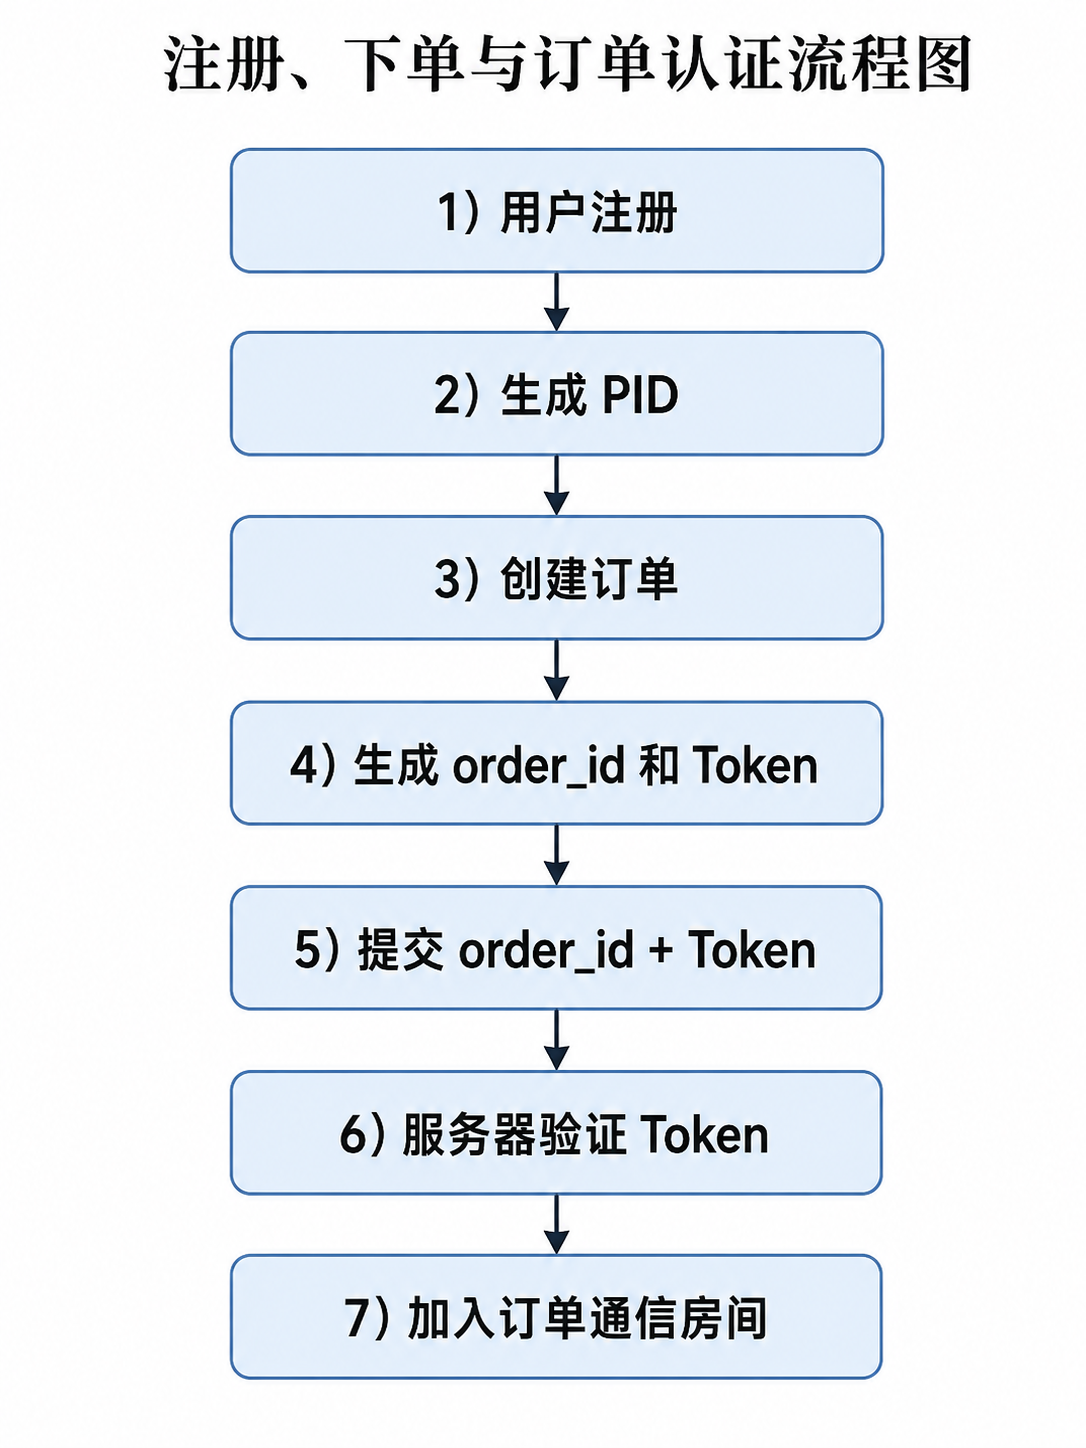
\includegraphics[width=0.8\textwidth]{content/chapter4/order_auth_flow.png}
    \caption{注册、下单与订单认证流程}
    \label{fig:order-auth-flow}
\end{figure}

该实现使订单号不再只是普通业务编号，而成为认证、通信、日志和溯源的统一索引。攻击者即使获得某个订单号，也无法在不知道合法 Token 的情况下进入对应通信通道，从而降低订单通信越权风险。
